\chapter[Lecture 5]{}\label{lec5}

\section*{Conjugate elements}

If $B$ and $C$ are conjugate to $A$; $B$ and $C$ are conjugate to each other.

\begin{proof}
\begin{xalignat*}{2}
B &= XAX^{-1} &\quad C&= YAY^{-1}\\[3pt]
\therefore\quad A&= Y^{-1}CY &\quad \therefore\quad B&= XY^{-1}CYX^{-1}=(XY^{-1})C(XY^{-1})^{-1}\\[3pt]
                 & &&\hspace{2.4cm} =ZCZ^{-1}
\end{xalignat*}

Here we assumed $(XY^{-1})^{-1}=(Y^{-1})^{-1}X^{-1}=YX^{-1}$

This can be proved as 
\begin{align*}
(AB^{-1})(AB)&=E\Rightarrow (AB^{-1})ABB^{-1}=EB^{-1}\\[3pt]
&\Rightarrow (AB)^{-1}AA^{-1}=B^{-1}A^{-1}\Rightarrow(AB)^{-1}=B^{-1}A^{-1}\\[3pt]
E &=(AB)^{-1}AB=(B^{-1}A^{-1})(AB)=B^{-1}(A^{-1})(A)B\\[3pt]
  &=B^{-1}B=E=(AB)^{-1}(AB)\\[3pt]
\therefore\quad & (AB)=B^{-1}A^{-1}
\end{align*}
\end{proof}

\subsection*{Class of elements}

All mutually conjugate elements form a class of elements.

E.g. A class including $A_{i}$ is found as
$$
EA_{i}E^{-1}=A_{i}; \ A_{2}A_{i}A^{-1}_{2};\ldots A_{h}A_{i}A^{-1}_{h}
$$
\begin{itemize}
\item In this way, we can divide a group into distinct {\bf classes}

\item One can form classes using symmetry considerations instead of using this tedious method.
\end{itemize}

\begin{example*}
Take symmetry operations of the triangle
\begin{align*}
\text{The classes are: } E &\to \text{ identity}\\
A,B,C &\to \text{ rotation by }\pi\\
D,F &\to \text{ rotation by } \dfrac{2\pi}{3}
\end{align*}
\begin{itemize}
\item $E$ is the only class, which is also a {\bf subgroup}.

\item In abelian group, each element is  a {\bf class}
$$
XA_{i}X^{-1}=A_{i}XX^{-1}=A_{i}
$$

\item If the group elements are represented by matrices, the {\bf trace}'s in a class is same for matrices $\to$ conjugation is similarity transformation that leaves {\bf trace} invariant.
\end{itemize}
\end{example*}

\subsection*{Physical meaning}

Group elements are covering operation of a symmetrical object.

Now, $B=X^{-1}AX$ may be interpreted as 

first rotate the object by $X$ to come to an equivalent position operate $A$

Then undo rotation $\Rightarrow$ rotate in reverse direction $(\overline{X}^{-1})$

$\therefore$ $B$ must be a similar kind of operation as $A$.

E.g., rotation by same angle but performed about some different axis which is related to axis of rotation of $A$ by $X^{-1}$

\begin{example*}
Conjugation of $A$ with $D$ i.e., $D^{-1}AD=C$
\begin{figure}[H]
\centering
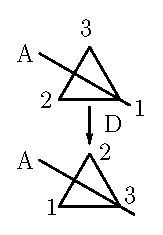
\includegraphics{images/lecture5/fig1.eps}
\end{figure}

$D$ rotates the triangle clockwise by $\dfrac{2\pi}{3}$ 

The operate
\begin{figure}[H]
\centering
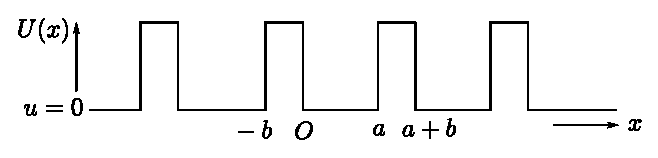
\includegraphics{images/lecture5/fig2.eps}
\end{figure}

Then operate $D^{-1}=F$
\begin{figure}[H]
\centering
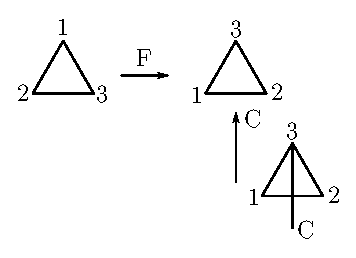
\includegraphics{images/lecture5/fig3.eps}
\end{figure}

This is equivalent to $C$ where the axis of rotation is the rotated anticlockwise $A$ rotation axis $(D^{-1})$.
\end{example*}

\subsection*{Invariant Subgroup}

If a subgroup $S$ consists entirely of complete classes, it is called an invariant subgroup or {\bf Normal Divisor}.

Complete class means $\to$ if $A\in S$ then all elements $X^{-1}AX$ for all $X$ are in $S$ even when $X\in \mathfrak{g}$ but $X\in S$.

{\bf Complex : \boldmath$k=(k_{1},k_{2}\ldots k_{n})\to$ a collection of group elements regardless of order.}

Let assume for Complexes : $\mathcal{K}X=(K_{1}X,K_{2}X,K_{3}X\ldots K_{n}X)$

(multiplication of complex by a group element)

$\mathcal{K}\mathcal{R}=(K_{1}R_{1},K_{1}R_{2},\ldots,K_{1}R_{m},\ldots,K_{n}R_{m})$

(multiplication by another complex)

Elements are considered to be included once, regardless of how often they are generated.

\eject

For simplicity, say {\bf sets of elements} as {\bf complex}es 
\begin{itemize}
\item Closure property $SS=S$

\item If $S$ is invariant subgroup then $X^{-1}SX=S$ for all $X\in \mathfrak{g}$

$\therefore$ \ $SX=XS\Rightarrow$ Left and Right cosets of invariant subgroup. $S$ are identical.
$$
\mathcal{K}_{i}=(K_{1},K_{2}\ldots, K_{n})
$$
\end{itemize}

\subsection*{Factor Group}
\begin{itemize}
\item In a group of order `$h$', `$S$' is a subgroup of order `$g$' and there are $(n-1)$ distinct cosets, each coset can be considered a a complex.

\item If $S$ is invariant subgroup, for a complex $\mathcal{K}_{i}$, we can write $\mathcal{K}_{i}=S\mathcal{K}_{i}=\mathcal{K}_{i}S$

N.B. $SK_{i}=SK_{j}$ if $K_{i}$ and $K_{j}$ are elements of $\mathcal{K}$ [we donot regard order] same coses.

\item Together with $S$ as an unit element and $(n-1)$ distinct cosets as $(n-1)$ elements one can define a group of order `$n$' $(n=\dfrac{h}{g})$ called {\bf Factor Group}.

\item In Factor group, $S$ behaves like an unit element.
\end{itemize}

$\mathcal{K}_{i}SK_{i}$ by definition of {\bf coset}.

\begin{proof}
$S\mathcal{K}_{i}=S(SK_{i})=(SS)K_{i}=SK_{i}=\mathcal{K}_{i}$

Follow Group multiplication rule:
$$
\mathcal{K}_{i}\mathcal{K}_{j}=(SK_{i})(SK_{j})=K_{i}SSK_{j}=K_{i}SK_{j}=S(K_{i}K_{j})=(\mathcal{K}_{i}\mathcal{K}_{j})
$$
where $(\mathcal{K}_{i}\mathcal{K}_{j})$ is a coset associated with the product $K_{i}K_{j}$.
\end{proof}

\subsection*{Isomorphy:}

Two groups having the same multiplication table are called isomorphic $\Rightarrow$ There is a one to one correspondence between the elements.

E.g., $A,B,C\ldots \in \mathfrak{g}$\quad $A',B',C'\ldots \in \mathfrak{g}'$

such that $AB=C$ implies $A'B'=C'$

\subsection*{Homomorphy:}

Two groups are called homomorphic if there is a correspondence both the elements of the two groups of the sort
\begin{align*}
& A\leftrightarrow A'_{1},A'_{2},A'_{3}\ldots\\
& B\leftrightarrow B'_{1},B'_{2},B'_{3}\ldots
\end{align*}
If $AB=C$, then product of any $A'_{i}$ and any $B'_{j}$ will produce $C'_{k}$

$\Rightarrow$ many to one correspondence.

E.g., Group $E$ i homomorphic to any other group.

\subsection*{Class multiplication}

Class $\to$ collection of mutually conjugate element.

In a complete class \fbox{$X^{-1}CX=C$}.

\begin{proof}
Each element on the left must appear on the right as they are conjugate to each other.

Class multiplication
\begin{align*}
C_{i}C_{j} &= X^{-1}C_{i}XX^{-1}C_{j}X\\
         &= X^{-1}(C_{i}C_{j})X\text{~ for all } X
\end{align*}
$$
a= \fbox{$C_{i}C_{j}=\sum\limits_{k}C_{ijk}C_{k}$}
$$
$C_{ijk}$ is an integer telling how often $C_{k}$ appears in the product $C_{i}C_{j}$.
\end{proof}

\begin{example*}
\begin{align*}
C_{1} &= E; C_{2}=A,B,C; C_{3}=D,F\\
C_{1}C_{2} &= C_{2}; C_{1}C_{3}=C_{3}\\
C_{2}C_{2} &= 3C_{1}+3C_{3}\quad C_{2}C_{3}=2C_{2}
\end{align*}
Look at the group multiplication table.
\begin{center}
\begin{tabular}{|>{$}c<{$}|>{$}c<{$}|>{$}c<{$}|>{$}c<{$}|>{$}c<{$}|>{$}c<{$}|>{$}c<{$}|}
\hline
 & E & A & B & C & D & F\\
\hline
E & E & A & B & C & D & F\\
\hline
A & A & E & D & F & B & C\\
\hline
B & B & F & E & D & C & A\\
\hline
C & C & D & F & E & A & B\\
\hline
D & D & C & A & B & F & E\\
\hline
F & F & B & C & A & E & D\\
\hline
\end{tabular}
\end{center}

For Triangle
\begin{figure}[H]
\centering
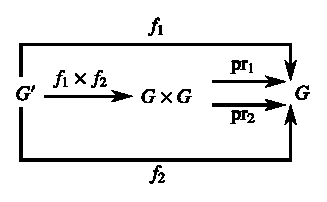
\includegraphics{images/lecture5/fig4.eps}
\end{figure}
\end{example*}
